\documentclass[remotesensing,article,submit,moreauthors,pdftex]{Definitions/mdpi} 

\firstpage{1} 
\makeatletter 
\setcounter{page}{\@firstpage} 
\makeatother
\pubvolume{1}
\issuenum{1}
\articlenumber{0}
\pubyear{2021}
\copyrightyear{2021}
\datereceived{} 
\dateaccepted{} 
\datepublished{} 
\hreflink{https://doi.org/}

\usepackage{breakcites}
\usepackage{float}
\usepackage{graphicx}
\usepackage{subcaption}
\usepackage{geometry}
\usepackage{amsmath}
\newcommand{\inlineeqnum}{\refstepcounter{equation}~~\mbox{(\theequation)}}
\usepackage{enumitem}
\usepackage[ruled,vlined]{algorithm2e}
\usepackage{booktabs}
\usepackage{pgfplotstable}
\pgfplotsset{compat=1.17}
\usepackage{longtable}
\usepackage{tabu}
\usepackage{hyperref}

\Title{
    Increasing the Effectiveness of Active Learning: Introducing Artificial
    Data Generation in Active Learning for Land Use/Land Cover Classification
}

% MDPI internal command: Title for citation in the left column
\TitleCitation{
    Increasing the Effectiveness of Active Learning: Introducing Artificial
    Data Generation in Active Learning for Land Use/Land Cover Classification
}

% Orcid ID
\newcommand{\orcidauthorA}{0000-0001-5889-3575}
\newcommand{\orcidauthorB}{0000-0001-7019-3782}
\newcommand{\orcidauthorC}{0000-0002-0834-0275}

\Author{
    Joao Fonseca $^{1,}$*\orcidA{},
    Georgios Douzas $^{1}$\orcidB{},
    Fernando Bacao $^{1}$\orcidC{}
}

% MDPI internal command: Authors, for metadata in PDF
\AuthorNames{Joao Fonseca, Georgios Douzas and Fernando Bacao}

% MDPI internal command: Authors, for citation in the left column
\AuthorCitation{Fonseca, J.; Douzas, G.; Bacao, F.}

\address{%
$^{1}$ \quad NOVA Information Management School (NOVA IMS), Universidade Nova
    de Lisboa, Campus de Campolide, 1070-312 Lisboa, Portugal;
    gdouzas@novaims.unl.pt (G.D.); bacao@novaims.unl.pt (F.B.)\\
    * \quad Correspondence: jpfonseca@novaims.unl.pt (J.F.)
}

\corres{Correspondence: jpfonseca@novaims.unl.pt}

\abstract{
    In remote sensing, Active Learning (AL) has become an important technique
    to collect informative ground truth data ``on-demand'' for supervised
    classification tasks. In spite of its effectiveness, it is still
    significantly reliant on user interaction, which makes it both expensive
    and time consuming to implement. Most of the current literature focuses on
    the optimization of AL by modifying the selection criteria and the
    classifiers used. Although improvements in these areas will result in more
    effective data collection, the use of artificial data sources to reduce
    human-computer interaction remains unexplored. In this paper, we introduce
    a new component to the typical AL framework, the data generator, a source
    of artificial data to reduce the amount of user-labeled data required in
    AL\@. The implementation of the proposed AL framework is done using
    Geometric SMOTE as data generator. We compare the new AL framework to the
    original one using similar acquisition functions and classifiers over
    three AL-specific performance metrics in seven benchmark datasets. We show
    that this modification of the AL framework significantly reduces cost and
    time requirements for a successful AL implementation in all of the
    datasets used in the experiment. 
}

\keyword{
    Active Learning;
    Artificial Data Generation;
    Land Use/Land Cover Classification; 
    Oversampling;
    SMOTE
}

\begin{document}

\section{Introduction}~\label{sec:introduction}

The technological development of air and spaceborne sensors, as well as the
increasing number of remote sensing missions have allowed the continuous
collection of large amounts of high quality remotely sensed data. This data is
often composed of multi and hyper spectral satellite imagery, essential for
numerous applications, such as Land Use/Land Cover (LULC) change detection,
ecosystem management~\cite{Nagai2020}, agricultural
management~\cite{Huang2018}, water resource management~\cite{Wang2018}, forest
management, and urban monitoring~\cite{Khatami2016}. Despite LULC maps being
essential for most of these applications, their production is still a
challenging task~\cite{Gavade2019, Wulder2018}. They can be updated using
one of the following strategies:

\begin{enumerate}
    \item Photo-interpretation. This approach consists of evaluating a patch's
        LULC class by a human operator based on orthophoto and satellite image
        interpretation~\cite{costa2020introducing}. This method guarantees a
        decent level of accuracy, as it is dependent on the interpreter's
        expertise and human error. Typically, it is an expensive,
        time-consuming task that requires the expertise of a
        photo-interpreter. This task is also frequently applied to obtain
        ground-truth labels for training and/or validating Machine Learning
        (ML) algorithms for related tasks~\cite{vermote2020remote,
        COSTANTINO2020}. 
    \item Automated mapping. This approach is based on the usage of a ML
        method or a combination of methods in order to obtain an updated LULC
        map. The development of a reliable automated method is still a
        challenge among the ML and remote sensing community, since the
        effectiveness of existing methods varies across applications and
        geographical areas~\cite{Gavade2019}. Typically, this method requires
        the existence of ground-truth data, which is frequently outdated or
        nonexistent for the required time frame~\cite{Nagai2020}. On the other
        hand, employing a ML method provides readily available and relatively
        inexpensive LULC maps. The increasing quality of state-of-the-art
        classification methods have motivated the application and adaptation
        of these methods in this domain~\cite{Maxwell2018}.
    \item Hybrid approaches. These approaches employ photo-interpreted data to
        augment the training dataset and improve the quality of automated
        mapping~\cite{Ruzicka2020}. It attempts to accelerate the
        photo-interpretation process by selecting a smaller sample of the
        study area to be interpreted. The goal is to minimize the inaccuracies
        found in the LULC map by supplying high-quality ground-truth data to
        the automated method. The final (photo-interpreted) dataset consists
        of only the most informative samples, \textit{i.e.}, patches that are
        typically difficult to classify for a traditional automated mapping
        method~\cite{Liu2020}. 
\end{enumerate}

The latter method is best know as AL\@. It is especially useful whenever there
is a shortage or even absence of ground-truth data and/or the mapping region
does not contain updated LULC maps~\cite{Su2020}. In a context of limited
sample-collection budget, the collection of the most informative samples
capable of optimally increasing the classification accuracy of a LULC map is
of particular interest~\cite{Su2020}. AL attempts to minimize the
human-computer interaction involved in photo-interpretation by selecting the
data points to include in the annotation process. These data points are
selected based on an uncertainty measure and represent the points close to the
decision borders. Afterwards, they are passed on for photo-interpretation and
added to the training dataset, while the points with the lowest uncertainty
values are ignored for photo-interpretation and classification. This process
is repeated until a convergence criterion is reached~\cite{Pasolli2016}. 

The relevant work developed within AL is described in detail in
Section~\ref{sec:al-sota}. This paper attempts to address some of the
challenges found in AL, mainly inherited from automated and photo-interpreted
mapping: mapping inaccuracies and time consuming human-computer interactions.
These challenges have different sources:

\begin{enumerate}
    \item Human error. The involvement of photo-interpreters in the data
        labeling step carries an additional risk to the creation of LULC
        patches. The minimum mapping unit being considered, as well as the
        quality of the orthophotos and satellite images being used, are some of
        the factors that may lead to the overlooking of small-area LULC patches
        and label-noisy training data~\cite{Pelletier2017}.
    \item High-dimensional datasets. Although the amount of bands
        (\textit{i.e.}, features) present in multi and hyper spectral images
        contain useful information for automated classification, they also
        introduce an increased level of complexity and redundancy in the
        classification step~\cite{Stromann2020}. These datasets are often
        prone to the Hughes phenomenon, also known as the curse of
        dimensionality. 
    \item Class separability. Producing an LULC map considering classes with
        similar spectral signatures makes them difficult to
        separate~\cite{Alonso-Sarria2019}. A lower pixel resolution of the
        satellite images may also imply mixed-class pixels, which may lead to
        both lower class separability as well as higher risk of human error.
    \item Existence of rare land cover classes. The varying morphologies of
        different geographical regions naturally implies an uneven distribution
        of land cover classes~\cite{Feng2018}. This is particularly relevant in
        the context of AL since the data selection method is based on a given
        uncertainty measure over data points whose class label is unknown.
        Consequently, AL's iterative process of data selection may disregard
        wrongly classified land cover areas belonging to a minority class.
\end{enumerate}

Research developed in the field of AL typically focus on the reduction of
human error by minimizing the human interaction with the process through the
development of more efficient choosers and selection criteria within the
generally accepted AL framework. Concurrently, the problem of rare land cover
classes is rarely addressed. This is a frequent problem in the ML community,
known as the Imbalanced Learning problem. This problem exists whenever there
is an uneven between-class distribution in the dataset~\cite{Chawla2004}.
Specifically, most classifiers are optimized and evaluted using accuracy-like
metrics, which are designed to work primarily with balanced datasets.
Consequently, these metrics tend to introduce a bias towards the majority
class by attributing an importance to each class proportional to its relative
frequency~\cite{Maxwell2018}. As an example, such a classifier could achieve
an overall accuracy of 99\% on a binary dataset where the minority class
represents 1\% of the overall dataset and still be useless. A number of
methods have been developed to deal with this problem. They can be categorized
into three different types of approaches~\cite{Fernandez2013,Kaur2019}.
Cost-sensitive solutions perform changes to the cost matrix in the learning
phase. Algorithmic level solutions modify specific classifiers to reinforce
learning on minority classes. Resampling solutions modify the dataset by
removing majority samples and/or generating artificial minority samples. The
latter is independent from the context and can be used alongside any
classifier. Because of this we will focus on artificial data generation
techniques, presented in Section~\ref{sec:ovs-sota}.

In this paper, we propose a novel AL framework to address two limitations
commonly found in the literature: minimize human-computer interaction and
reduce the class imbalance bias. This is done with the introduction of an
additional component in the iterative AL procedure (the generator), used to
generate artificial data to both balance and augment the training dataset. The
introduction of this component is expected to reduce the number of iterations
required until convergence of the classifier's quality.

This paper is organized as follows: Section~\ref{sec:introduction} explains
the problem and its context, Sections~\ref{sec:al-sota} and~\ref{sec:ovs-sota}
describe the state of the art in AL and Oversampling techniques,
Section~\ref{sec:proposed-method} explains the proposed method,
Section~\ref{sec:methodology} covers the datasets, evaluation metrics, ML
classifiers and experimental procedure, Section~\ref{sec:results} presents the
experiment's results and discussion and Section~\ref{sec:conclusion} presents
the conclusions drawn from our findings.

\section{Active Learning Approaches}~\label{sec:al-sota}

As the amount of unlabeled data increases, the interest and practical
usefulness of AL follows that trend~\cite{Kottke2017}. AL is used as the
general definition of frameworks aiming to train a learning system in multiple
steps, where a set of new data points are chosen and added to the training
dataset each time~\cite{Ruzicka2020}. Typically, an AL framework is composed
of the following elements~\cite{Sverchkov2017,Su2020,Ruzicka2020}:

\begin{enumerate}
    \item Unlabeled dataset. Consists of the original data source (or a sample
        thereof). It is used in combination with the chooser and the selection
        criterion to expand the training set in regions where the
        classification uncertainty is higher. Therefore, this dataset is used
        for both producing the initial training sample by selecting a set of
        observations for the supervisor to annotate (discussed in point 3) and
        calculating the uncertainty map to augment the training dataset.
    \item Supervisor. An external entity to which the uncertainty map is
        presented to. The supervisor is responsible for annotating unlabeled
        instances to be added to the augmented dataset. In remote sensing, the
        supervisor is typically a photo-interpreter, as is the case
        in~\cite{li2020}. Some of the research also refers to the supervisor
        as the \textit{oracle}~\cite{Ruzicka2020, Yoo2019, Aghdam2019,
        Cawley2011}.
    \item Initial training dataset. It is a small sample of data used to
        initiate the first AL iteration. The size of the initial training
        sample normally varies between no instances at all and
        10\%~\cite{Li2013}.
    \item Current and expanded training dataset. It is the concatenation of
        the initial training and the datasets labeled by the supervisor in
        past iterations (discussed in point 2).
    \item Chooser (classifier). Produces the class probabilities for each
        unlabeled instance.
    \item Selection criterion. It quantifies the chooser's uncertainty level
        for each instance belonging to the unlabeled dataset. It is typically
        based on the class probabilities assigned by the chooser. In some
        situations, the chooser and the selection criterion are grouped
        together under the concept \textit{acquisition
        function}~\cite{Ruzicka2020} or \textit{query function}~\cite{Su2020}.
        Some of the literature refers to the selection criterion by using the
        concept \textit{sampling scheme}~\cite{Liu2020}.
\end{enumerate}

Figure~\ref{fig:al_typical} schematizes the steps involved in a complete AL
iteration. For a better context within the remote sensing domain, the
prediction output is identified as the LULC map. This framework starts by
collecting unlabeled data from the original data source. It is used to
generate a random initial training sample and is labeled by the supervisor. In
practical applications, the supervisor is frequently a group of
photo-interpreters~\cite{Kottke2017}. The chooser is trained on the resulting
dataset and is used to predict the class probabilities on the unlabeled
dataset. The class probabilities are fed into a selection criterion to
estimate the prediction's uncertainty, out of which the instances with the
highest uncertainty will be selected. This calculation is motivated by the
absence of labels in the uncertainty dataset. Therefore, it is impossible to
estimate the prediction's accuracy in the unlabeled dataset in a real case
scenario. The iteration is completed when the selected points are tagged by
the supervisor and added to the training dataset (\textit{i.e.}, the augmented
dataset). 

\begin{figure}[htb]
	\centering
	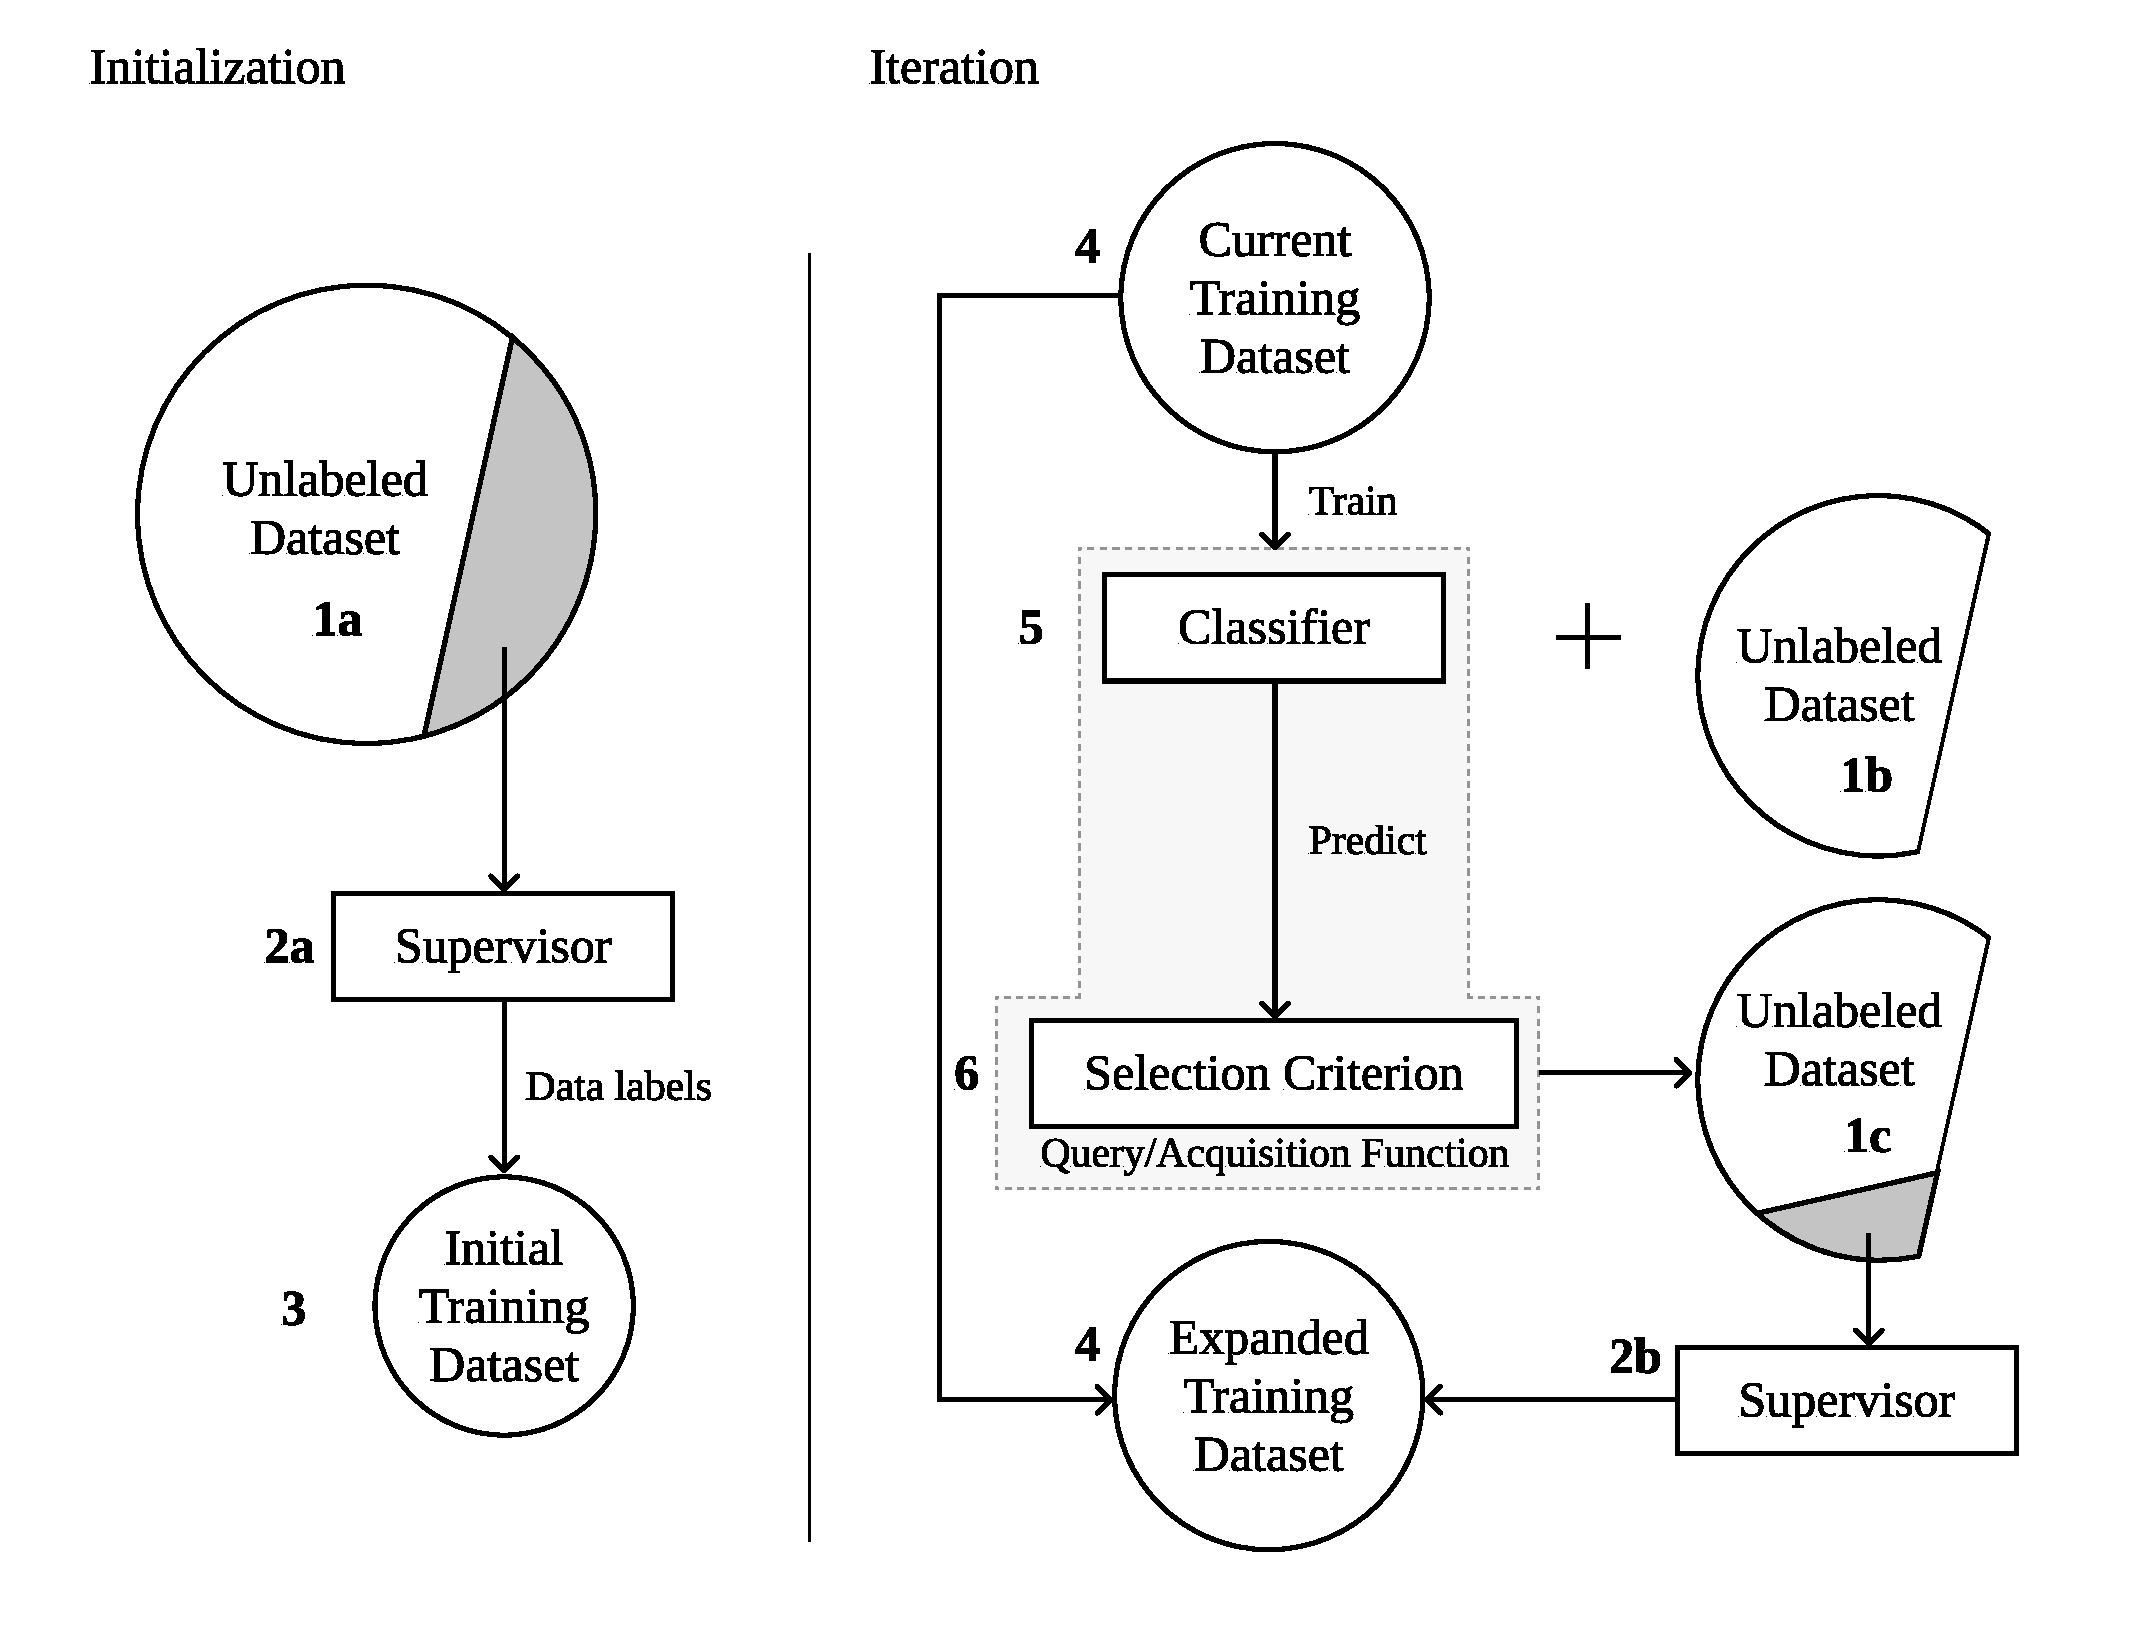
\includegraphics[width=\linewidth]{../analysis/al_typical}
	\caption{Diagram depicting the typical AL framework.
    }~\label{fig:al_typical}
\end{figure}

A common challenge found in AL tasks is ensuring the consistency of AL over
different initializations~\cite{Kottke2017}. There are two factors involved in
this phenomenon. On one hand, the implementation of the same method over
different initializations may result in significantly different initial
training samples, amounts to varying accuracy curves. On the other hand, the
lack of a robust selection criterion and/or chooser may also result in
inconsistencies across AL experiments with different initializations. This
phenomenon was observed and documented in a LULC classification context
in~\cite{tuia2011using}.

Selecting an efficient selection criterion is particularly important to find
the instances closest to the decision border (\textit{i.e.}, instances
difficult to classify)~\cite{Shrivastava2021}. Therefore, most of AL related
studies focus on the design of the query/acquisition function~\cite{Su2020}.

\subsection{Non-informed selection criteria}

Only one non-informed (\textit{i.e.}, random) selection criterion was found in
the literature. Random sampling selects unlabeled instances without
considering any external information produced by the chooser. Since the method
for selecting the unlabeled instances is random, this method disregards the
usage of a chooser and is comparatively worse than any other selection
criterion. However, random sampling is still a powerful baseline
method~\cite{Cawley2011}. 

\subsection{Ensemble-based selection criteria}

Ensemble disagreement is based on the class predictions of a set of
classifiers. The disagreement between all the predictions for a given
instance is a common measure for uncertainty, although computationally
inefficient~\cite{Ruzicka2020,Pasolli2016}. It is calculated using the set of
classifications over a single instance, given by the number of votes
assigned to the most frequent class~\cite{Shrivastava2021}. This method was
implemented successfully for complex applications such as deep active
learning~\cite{Ruzicka2020}.

Multiview~\cite{Muslea2006} consists on the training of multiple independent
classifiers using different views, which correspond to the selection of subsets
of features or instances in the dataset. Therefore, it can be seen as a
bootstrap aggregation (bagging) ensemble disagreement method. It is represented
by the maximum disagreement score out of set of disagreements calculated for
each view~\cite{Shrivastava2021}. A lower value for this metric means a higher
classification uncertainty. Multiview-based maximum disagreement has been
successfully applied to hyper-spectral image classification in~\cite{Di2012}
and~\cite{Zhou2014}.

An adapted disagreement criterion for an ensemble of $k$-nearest neighbors has
been proposed in~\cite{Pasolli2016}. This method employs a $k$-nearest
neighbors classifier and computes an instance's classification uncertainty
based on the neighbors' class frequency using the maximum disagreement metric
over varying values for $k$. As a result, this method is comparable to
computing the dominant class' score over a weighted $k$-nearest neighbors
classifier. This method was also used on a multimetric active learning
framework~\cite{Zhang2016}.

Another relevant ensemble-based selection criterion is the binary random
forest-based query model~\cite{Su2020}. This method employs a one-versus-one
ensemble method to demonstrate an efficient data selection method using the
estimated probability of each binary random forest and determining the
classification uncertainty based on the probabilities closest to 0.5
(\textit{i.e.}, the least separable pair of classes are used to determine the
uncertainty value). However, this study fails to compare the proposed method
with other benchmark methods, such as random sampling.

\subsection{Entropy-based criteria}

A number of contributions have focused on entropy-based querying. The
application of entropy is common among active deep learning
applications~\cite{Aghdam2019}, where the training of an ensemble of
classifiers is often too expensive. 

Entropy query-by-bagging (EQB), also defined as maximum
entropy~\cite{Liu2020}, is an ensemble approach of the entropy selection
criterion, originally proposed in~\cite{Tuia2009}. This strategy uses the set
of predictions produced by the ensemble classifier to calculate those many
entropy measurements. The estimated uncertainty measure for one instance is
given by the maximum entropy within that set. EQB was observed to be an
efficient selection criterion. Specifically,~\cite{Shrivastava2021} applied
EQB on hyper-spectral remote sensing imagery using Support Vector Machines
(SVM) and Extreme Learning Machines (ELM) as choosers, achieving optimal
results when combining EQB with ELM\@. Another study successfully implemented
this method on an active deep learning application~\cite{Liu2020}. Another
study improved over this method with a normalized EQB selection
criterion~\cite{Copa2010}.

\subsection{Other relevant criteria}

Margin Sampling is a SVM-specific criterion, based on the distance of a given
point to the SVM's decision boundary~\cite{Shrivastava2021}. This method is
less popular than the remaining methods because it is limited to one type of
chooser (SVMs). One extension of this method is the multiclass level
uncertainty~\cite{Shrivastava2021}, calculated by subtracting the instance's
distance to the decision boundaries of the two most probable
classes~\cite{Demir2011}.

The Mutual Information-based (MI) criterion selects the new training instances
by maximizing the mutual information between the classifier and class labels
in order to select instances from regions that are difficult to classify.
Although this method is commonly used, it is frequently outperformed by the
breaking ties selection criterion~\cite{Li2011,Liu2018}.

The breaking ties (BT) selection criterion was originally introduced
in~\cite{Luo2003}. It consists of the subtraction between the probabilities of
the two most likely classes. Another related method is Modified Breaking Ties
scheme (MBT), which aims at finding the instances containing the largest
probabilities for the dominant class~\cite{Liu2018,Li2013a}

Another type of selection criteria identified is the loss prediction
method~\cite{Yoo2019}. This method replaces the selection criterion with a
predictor whose goal is to estimate the chooser's loss for a given
prediction. This allows the new classifier to estimate the prediction loss on
unlabeled instances and select the ones with the highest predicted loss.

Some of the literature fails to specify the strategy employed, although
inferring it is generally intuitive. For example,~\cite{Ertekin2007}
successfully used AL to address the imbalanced learning problem. They employed
an ensemble of SVMs as the chooser, as well as an ensemble-based selection
criterion. All of the research found related to this topic focused on the
improvement of AL through modifications on the selection criterion and
classifiers used. None of these publications proposed significant variations
to the original AL framework.

\section{Proposed method}~\label{sec:proposed-method}

Within the literature identified, most of the work developed in the AL domain
revolved around improving the quality of classification algorithms and/or
selection criteria. Although these methods allow earlier convergence of the
AL iterative process, the impact of these methods are only observed between
iterations. Consequently, none of these contributions focused on the
definition of decision borders within iterations. The method proposed in this
paper modifies the AL framework by introducing an artificial data generation
step within AL's iterative process. We define this component as the generator
and is intended to be integrated into the AL framework as shown in
Figure~\ref{fig:al_new}. 

This modification, by using a new source of data to augment the training set,
leverages the data annotation work conducted by the human operator. The
artificial data that is generated between iterations reduces the amount of
labeled data required to reach optimal performance and lower the amount of
human labor required to train a classifier to its optimal performance. This
process lowers the annotation and overall training costs by translating some
of the annotation cost into computational cost.

\begin{figure}[htb]
	\centering
	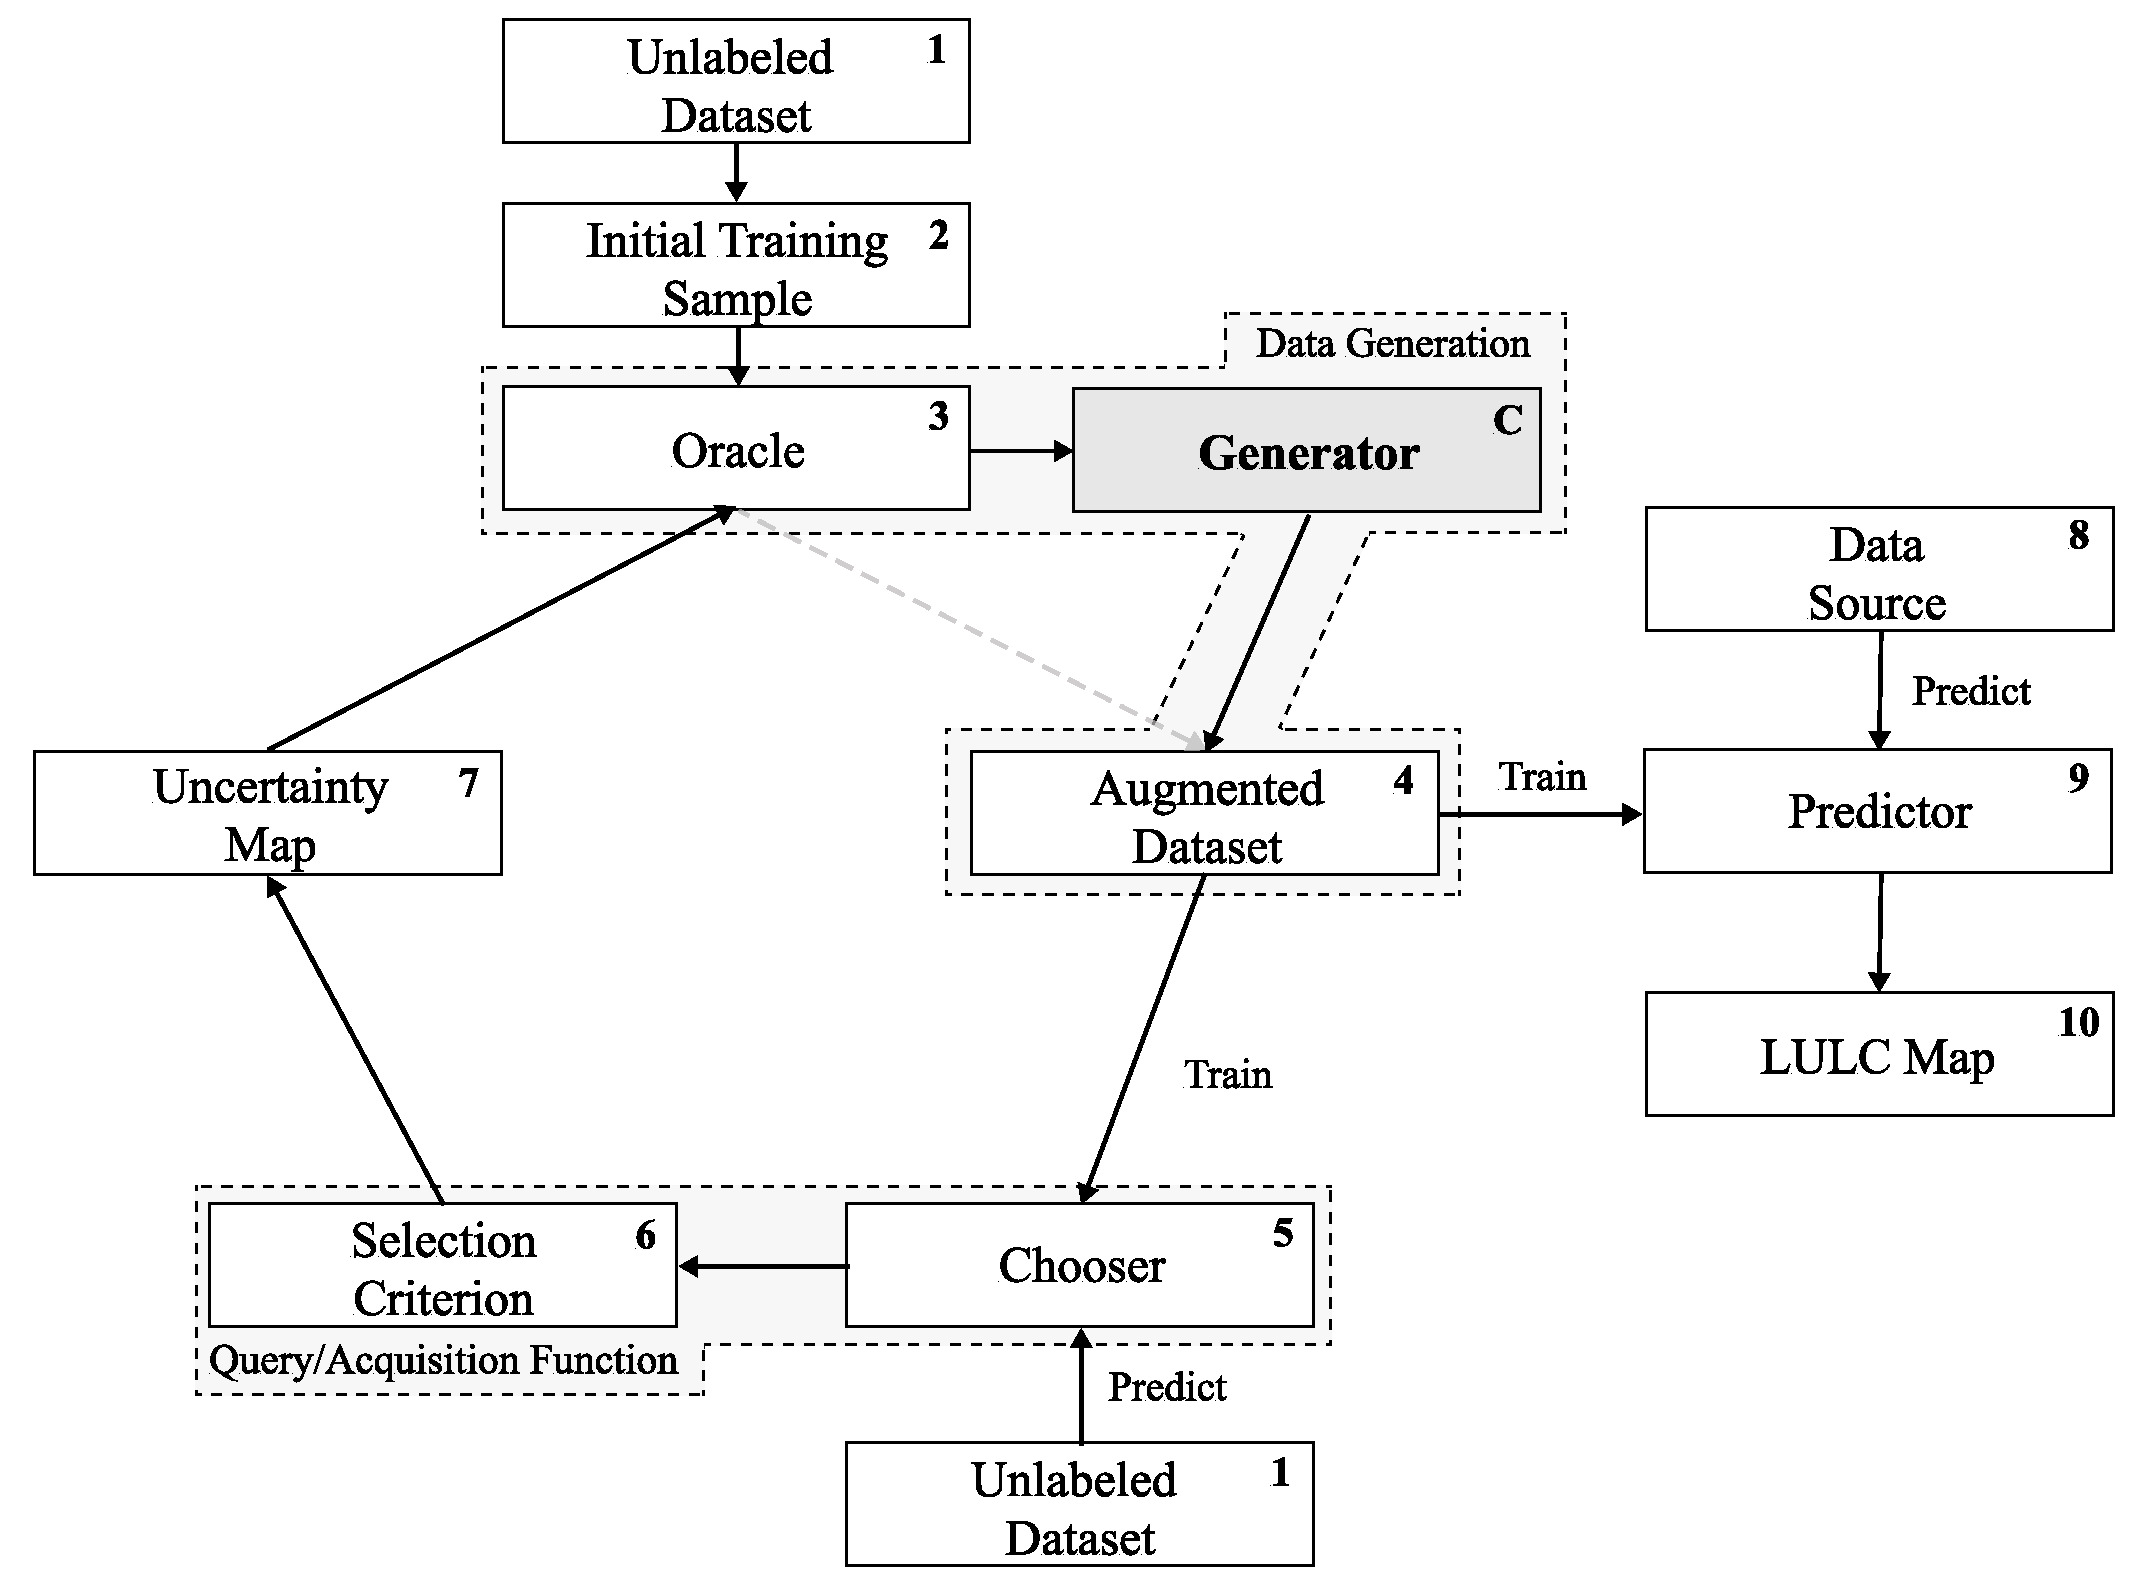
\includegraphics[width=\linewidth]{../analysis/al_new}
    \caption{Proposed AL framework. The data generation mechanism is
        represented as the generator (marked with~\textit{C}), which is used to add artificial
        instances to the data generation phase. The remaining steps are left
        unchanged.
    }~\label{fig:al_new}
\end{figure}

This method leverages the capability of artificial data to introduce more data
variability into the augmented dataset and facilitate the chooser's training
phase with a more consistent definition of the decision boundaries at each
iteration. Therefore, any algorithm capable of producing artificial data, be
it agnostic or specific to the domain, can be employed. The artificial data is
only used to train the classifiers involved in the process and is discarded
once the training phase is completed. The remaining steps in the AL framework
remain unchanged. This method addresses the limitations found in the previous
sections:

\begin{enumerate}
    \item The convergence of classification performance should be anticipated
        with the clearer definition of the decision boundaries across
        iterations.
    \item Annotation cost is expected to reduce as the need for labeled
        instances reduces along with the early convergence of the
        classification performance.
    \item The class imbalance bias observed in typical classification tasks, as
        well as in AL is mitigated by balancing the class frequencies at each
        iteration.
\end{enumerate}

Although the performance of this method is shown within a LULC classification
context, the proposed framework is independent from the domain. The high
dimensionality of remotely sensed imagery make its classification particularly
challenging when the availability of labeled data is scarce and/or comes at a
high cost, being subjected to the curse of dimensionality. Consequently, it is
a relevant and appropriate domain to test this method.

\section{Artificial Data Generation Approaches}~\label{sec:ovs-sota}

The generation of artificial data is a common approach to address imbalanced
learning tasks~\cite{Kaur2019}, as well as improving the effectiveness of
supervised learning tasks~\cite{DeVries2017}. In recent years some
sophisticated data generation approaches were developed. However, the scope of
this work is to propose the integration of a generator within the AL
framework. To do this, we will focus on heuristic data generation approaches,
specifically, oversamplers.

Heuristic data resampling methods employ local and/or global information to
generate new, relevant, non-duplicate instances. These methods are most
commonly used to populate minority classes and balance the between-class
distribution of a dataset. The Synthetic Minority Oversampling Technique
(SMOTE)~\cite{Chawla2002} is a popular heuristic oversampling algorithm,
proposed in 2002. The simplicity and effectiveness of this method contributes
to its prevailing popularity. It generates a new instance through a linear
interpolation of a randomly selected minority-class instance and one of its
randomly selected $k$-nearest neighbors. The implementation of SMOTE for LULC
classification tasks has been found to improve the quality of the predictors
used~\cite{Jozdani2019,Bogner2018}. Despite its popularity, its drawbacks
motivated the development of other oversampling methods~\cite{Douzas2019}.

Geometric SMOTE (G-SMOTE)~\cite{Douzas2019} introduces a modification of the
SMOTE algorithm in the data generation mechanism to produce artificial
instances with higher variability. Instead of generating artificial data as a
linear combination of the parent instances, it is done within a deformed,
truncated hyper-spheroid. G-SMOTE generates an artificial instance
$\overrightarrow{z}$ within a hyper-spheroid, formed by selecting a minority
instance $\overrightarrow{x}$ and one of its nearest neighbors
$\overrightarrow{y}$, as shown in Figure~\ref{fig:data_generation}. The
truncation and deformation parameters define the shape of the spheroid's
geometry. The method also modifies the selection strategy for the $k$-nearest
neighbors, accepting the generation of artificial instances using instances
from different classes, as shown in Figure~\ref{fig:data_generation}d. The
modification of both selection and generation mechanisms addresses the main
drawbacks found in SMOTE, the generation of both noisy data (\textit{i.e.,}
generate minority class instances within majority class regions) and
near-duplicate minority class instances~\cite{Douzas2019}. G-SMOTE has shown
superior performance when compared with other oversampling methods for LULC
classification tasks, regardless of the classifier sed~\cite{Douzas2019class}.

\begin{figure}[htb]
	\centering
	\includegraphics[width=.6\linewidth]{../analysis/data_generation}
    \caption{Example of G-SMOTE's generation process. G-SMOTE randomly selects
        instance $\protect\overrightarrow{x}$ and one of its nearest neighbors
        $\protect\overrightarrow{y}$ to produce instance
        $\protect\overrightarrow{z}$.
    }~\label{fig:data_generation}
\end{figure}

\section{Methodology}~\label{sec:methodology}

In this section we describe the datasets, evaluation metrics, oversampler,
classifiers, software used and the procedure developed. We demonstrate the
proposed method's efficiency over 7 datasets, sampled from publicly available,
well-known remote sensing hyperspectral scenes frequently found in remote
sensing literature. The datasets and sampling strategy are described in
Subsection~\ref{sec:datasets}. On each of these datasets, we apply 3 different
classifiers over the entire training set to estimate the optimal
classification performance, the original AL framework as the baseline
reference and the proposed method using G-SMOTE as a generator, described in
Subsection~\ref{sec:machine_learning_algorithms}. The metrics used to estimate
the performance of these algorithms are described in
Subsection~\ref{sec:evaluation_metrics}. Finally, the experimental procedure
is described in Subsection~\ref{sec:experimental_procedure}. 

Our methodology focuses on two objectives: (1) Comparison of optimal
classification performance among active learners and traditional supervised
learning and (2) Comparison of classification convergence efficiency among AL
frameworks.

\subsection{Datasets}~\label{sec:datasets}

The datasets used were extracted from publicly available repositories
containing hyperspectral images and groud truth data. Additionally, all
datasets were collected using the same sampling procedure. The description of
the hyperspectral scenes used in this study is provided in
Table~\ref{tab:rs_scene_description}. These scenes were chosen because of
their popularity in the research community and their high baseline
classification scores. Consequently, demonstrating an outperforming method in
this context is particularly challenging and valuable.

\end{paracol}
\begin{table}
    \centering
    \pgfplotstabletypeset[
    	begin table=\begin{longtable},
    	end table=\end{longtable},
        col sep=semicolon,
        string type,
        every head row/.style={%
            before row=\toprule,
            after row=\midrule
        },
        every last row/.style={after row=\bottomrule},
        string type,
    ]{../analysis/rs_scene_description.csv}
    \vspace{.2cm}
    \caption{\label{tab:rs_scene_description}
        Description of the hyperspectral scenes used in this experiment. The
        column ``Res. (m)'' refers to the resolution of the sensors (in
        meters) that captured each of the scenes.
    }
\end{table}
\begin{paracol}{2}
\linenumbers
\switchcolumn

The Indian Pines scene~\cite{Baumgardner2015} is composed of agriculture fields
in approximately two thirds of its coverage, low density buildup areas and
natural perennial vegetation in the remainder of its area (see
Figure~\ref{fig:indian_pines}). The Pavia Centre and University scenes are
hyperspectral, high-resolution images containing ground truth data composed of
urban-related coverage (see Figures~\ref{fig:pavia_centre}
and~\ref{fig:pavia_university}). The Salinas and Salinas A scenes contain
at-sensor radiance data. As subset of Salinas, the Salinas A scene contains
contains the vegetables fields present in Salinas and the latter is also
composed of bare soils and vineyard fields (see Figures~\ref{fig:salinas}
and~\ref{fig:salinas_a}). The Botswana scene contains ground truth data
composed of seasonal swamps, occasional swamps, and drier woodlands located in
the distal portion of the Delta (see Figure~\ref{fig:botswana}). The Kennedy
Space Center scene contains a ground truth composed of both vegetation and
urban-related coverage (see Figure~\ref{fig:kennedy_space_center})

\pagebreak
\end{paracol}
\begin{figure}[H]
	\centering 
	\begin{subfigure}{.24\textwidth}
		\centering
        \captionsetup{justification=centering}
		\includegraphics[height=1.5\linewidth]{../analysis/indian_pines}
		\subcaption{{\medbreak}}\label{fig:indian_pines}
	\end{subfigure}
	\begin{subfigure}{.24\textwidth}
		\centering
        \captionsetup{justification=centering}
		\includegraphics[height=1.5\linewidth]{../analysis/pavia_centre}
		\subcaption{{\medbreak}}\label{fig:pavia_centre}
	\end{subfigure}
	\begin{subfigure}{.24\textwidth}
		\centering
        \captionsetup{justification=centering}
		\includegraphics[height=1.5\linewidth]{../analysis/pavia_university}
		\subcaption{{\medbreak}}\label{fig:pavia_university}
	\end{subfigure}

	\begin{subfigure}{.24\textwidth}
		\centering
        \captionsetup{justification=centering}
		\includegraphics[height=1.5\linewidth]{../analysis/salinas}
		\subcaption{{\medbreak}}\label{fig:salinas}
	\end{subfigure}
	\begin{subfigure}{.24\textwidth}
		\centering
        \captionsetup{justification=centering}
		\includegraphics[height=1.5\linewidth]{../analysis/salinas_a}
		\subcaption{{\medbreak}}\label{fig:salinas_a}
	\end{subfigure}
	\begin{subfigure}{.24\textwidth}
		\centering
        \captionsetup{justification=centering}
		\includegraphics[height=1.5\linewidth]{../analysis/botswana}
		\subcaption{{\medbreak}}\label{fig:botswana}
	\end{subfigure}
	\begin{subfigure}{.24\textwidth}
		\centering
        \captionsetup{justification=centering}
		\includegraphics[height=1.5\linewidth]{../analysis/kennedy_space_center}
		\subcaption{{\medbreak}}\label{fig:kennedy_space_center}
	\end{subfigure}
    \caption{Gray scale visualization of a band (top row) and ground truth
        (bottom row) of each scene used in this study. (a) Indian Pines, (b)
        Pavia Centre, (c) Pavia University, (d) Salinas, (e) Salinas A, (f)
        Botswana, (g) Kennedy Space Center }\label{fig:scenes}
\end{figure}
\begin{paracol}{2}
\linenumbers
\switchcolumn

The sampling strategy is similar to all datasets. The pixels without a ground
truth label are first discarded. All the classes with cardinality lower than
150 are also discarded. This is done to maintain feasible Imbalance Ratios (IR)
across datasets (where $IR = \frac{count(C_{maj})}{count(C_{min})}$). Finally,
a stratified sample of 1500 instances are selected for the experiment. The
resulting datasets are described in Table~\ref{tab:datasets_description}. The
motivation for this strategy is three fold: (1) reduce the datasets to a
manageable size and allow the experimental procedure to be completed within a
feasible time frame, (2) ensure the relative class frequencies in the scenes
are preserved and (3) ensure equivalent analyses across datasets and AL
frameworks. In this context, a fixed number of instances per dataset is
especially important to standardize the AL-related performance metrics.

\end{paracol}
\begin{table}
    \centering
    \addtolength{\leftskip} {-2cm}
    \addtolength{\rightskip}{-2cm}
    \pgfplotstabletypeset[
        col sep=comma,
        string type,
        every head row/.style={%
            before row=\toprule,
            after row=\midrule
        },
        every last row/.style={after row=\bottomrule},
    ]{../analysis/datasets_description.csv}
    \caption{\label{tab:datasets_description}
        Description of the datasets collected from each corresponding scene.
        The sampling strategy is similar to all scenes.
    }
\end{table}
\begin{paracol}{2}
\linenumbers
\switchcolumn

\subsection{Machine Learning Algorithms}~\label{sec:machine_learning_algorithms}

We use two different types of ML algorithms. A data generation algorithm, used
to form the generator, and classification algorithms, used to calculate the
classification uncertainties in the unlabeled dataset and predict the class
labels in the validation and test sets.

Although any method capable of generating artificial data can be used as a
generator, the one used in this experiment is an oversampler, originally
developed to deal with imbalanced learning problems. Specifically, we chose
G-SMOTE, a state-of-the-art oversampler.

Three classification algorithms are used. We use different types of
classifiers to test the framework's performance under varying situations:
neighbors-based, linear and ensemble models. The neighbors-based classifier
chosen was $K$-nearest neighbors (KNN)~\cite{Cover1967}, a logistic regression
(LR)~\cite{Nelder1972} is used as the linear model and a random forest
classifier (RFC)~\cite{Ho1995} was used as the ensemble model.

The acquisition function is completed by testing three different selection
criteria. Random selection is used as a baseline selection criterion, whereas
entropy and breaking ties are used due to their popularity and independence of
the classifier used.

\subsection{Evaluation Metrics}~\label{sec:evaluation_metrics}

Since the datasets used in this experiment have an imbalanced distribution of
class frequencies, metrics such as the \textit{Overall Accuracy} (OA) and
\textit{Kappa coefficient} are insufficient to accurately depict
classification performance~\cite{Olofsson2013, Pontius2011}. Instead, metrics
such as Producer's Accuracy (or \textit{Recall}) and User's Accuracy (or
\textit{Precision}) can be used. Since they consist of ratios based on
True/False Positives (TP and FP) and Negatives (TN and FN), they provide per
class information regarding the classifier's classification performance.
However, in this experiment, the meaning and number of classes available in
each dataset varies, making these metrics difficult to synthesize.

The performance metric \textit{Geometric mean} (G-mean) is less
sensitive to the data imbalance bias~\cite{Jeni2013, Kubat1997}. Therefore, we
employ the G-mean scorer. It consists of the geometric mean of $Specificity =
\frac{TN}{TN + FP}$ and $Sensitivity = \frac{TP}{TP+FN}$ (also known as
\textit{Recall})~\cite{Kubat1997}. Both metrics are calculated in a multiclass
context considering a one-versus-all approach. For multiclass problems, the
\textit{G-mean} scorer is calculated as its average per class values: 
        
\begin{equation*}
    \textit{G-mean} = \sqrt{\overline{Sensitivity}_i \times
    \overline{Specificity}_i}
\end{equation*}
    
The comparison of classification convergence across AL frameworks and
selection criteria is done using 2 AL-specific performance metrics.
Particularly, we follow the recommendations found in~\cite{Kottke2017}. Each
AL configuration is evaluated using the \textit{Area Under the Learning Curve}
(AULC) performance metric. It is the sum of the classification performance
values of all iterations. To facilitate the analysis of the results, we fix
the range of this metric between $[0,1]$ by dividing it with the total amount
of iterations (\textit{i.e.}, the maximum performance area). 

The \textit{Data Utilization Rate} (DUR)~\cite{Reitmaier2013} metric consists
of the ratio between the number of instances required to reach a given G-mean
score threshold by an AL strategy and an equivalent baseline strategy. For
easier interpretability, we simplify this metric by using the percentage
of training data used by an AL strategy to reach the performance threshold,
instead of presenting these values as a ratio of the baseline strategy. The
DUR metric is measured at 9 different performance levels, between
0.6 and 0.95 G-mean scores at a 0.05 step.

\subsection{Experimental Procedure}~\label{sec:experimental_procedure}

A common practice in methodological evaluations is the implementation of an
offline experiment~\cite{Kagy2019}. It consists of using an existing set of
labeled data as a proxy for the population of unlabeled instances. Because the
dataset is already fully labeled, the supervisor's typical annotation process
involved in each iteration is done at zero cost. Each AL and classifier
configuration is tested using a stratified 5-fold cross validation testing
scheme. For each round, the larger partition is split in a stratified fashion
to form a training and validation set (containing 20\% of the original
partition). The validation set is used to evaluate the convergence efficiency
of active learners; the chooser's classification performance metrics and
amount of data points used at each iteration are used to compute the AULC and
DUR\@. Additionally, within the AL iterative process, the classifier with
optimal performance on the validation set is evaluated using the test set. In
order to further reduce possible initialization biases, this procedure is
repeated 3 times with different initialization seeds and the results of all
runs are averaged (\textit{i.e.}, each configuration is trained and evaluated
15 times). Finally, the maximum performance lines are calculated using the
same approach. In those cases, the validation set is not used. The
experimental procedure is depicted in Figure~\ref{fig:experiment_pipeline}.

\end{paracol}
\begin{figure}[H]
	\centering
	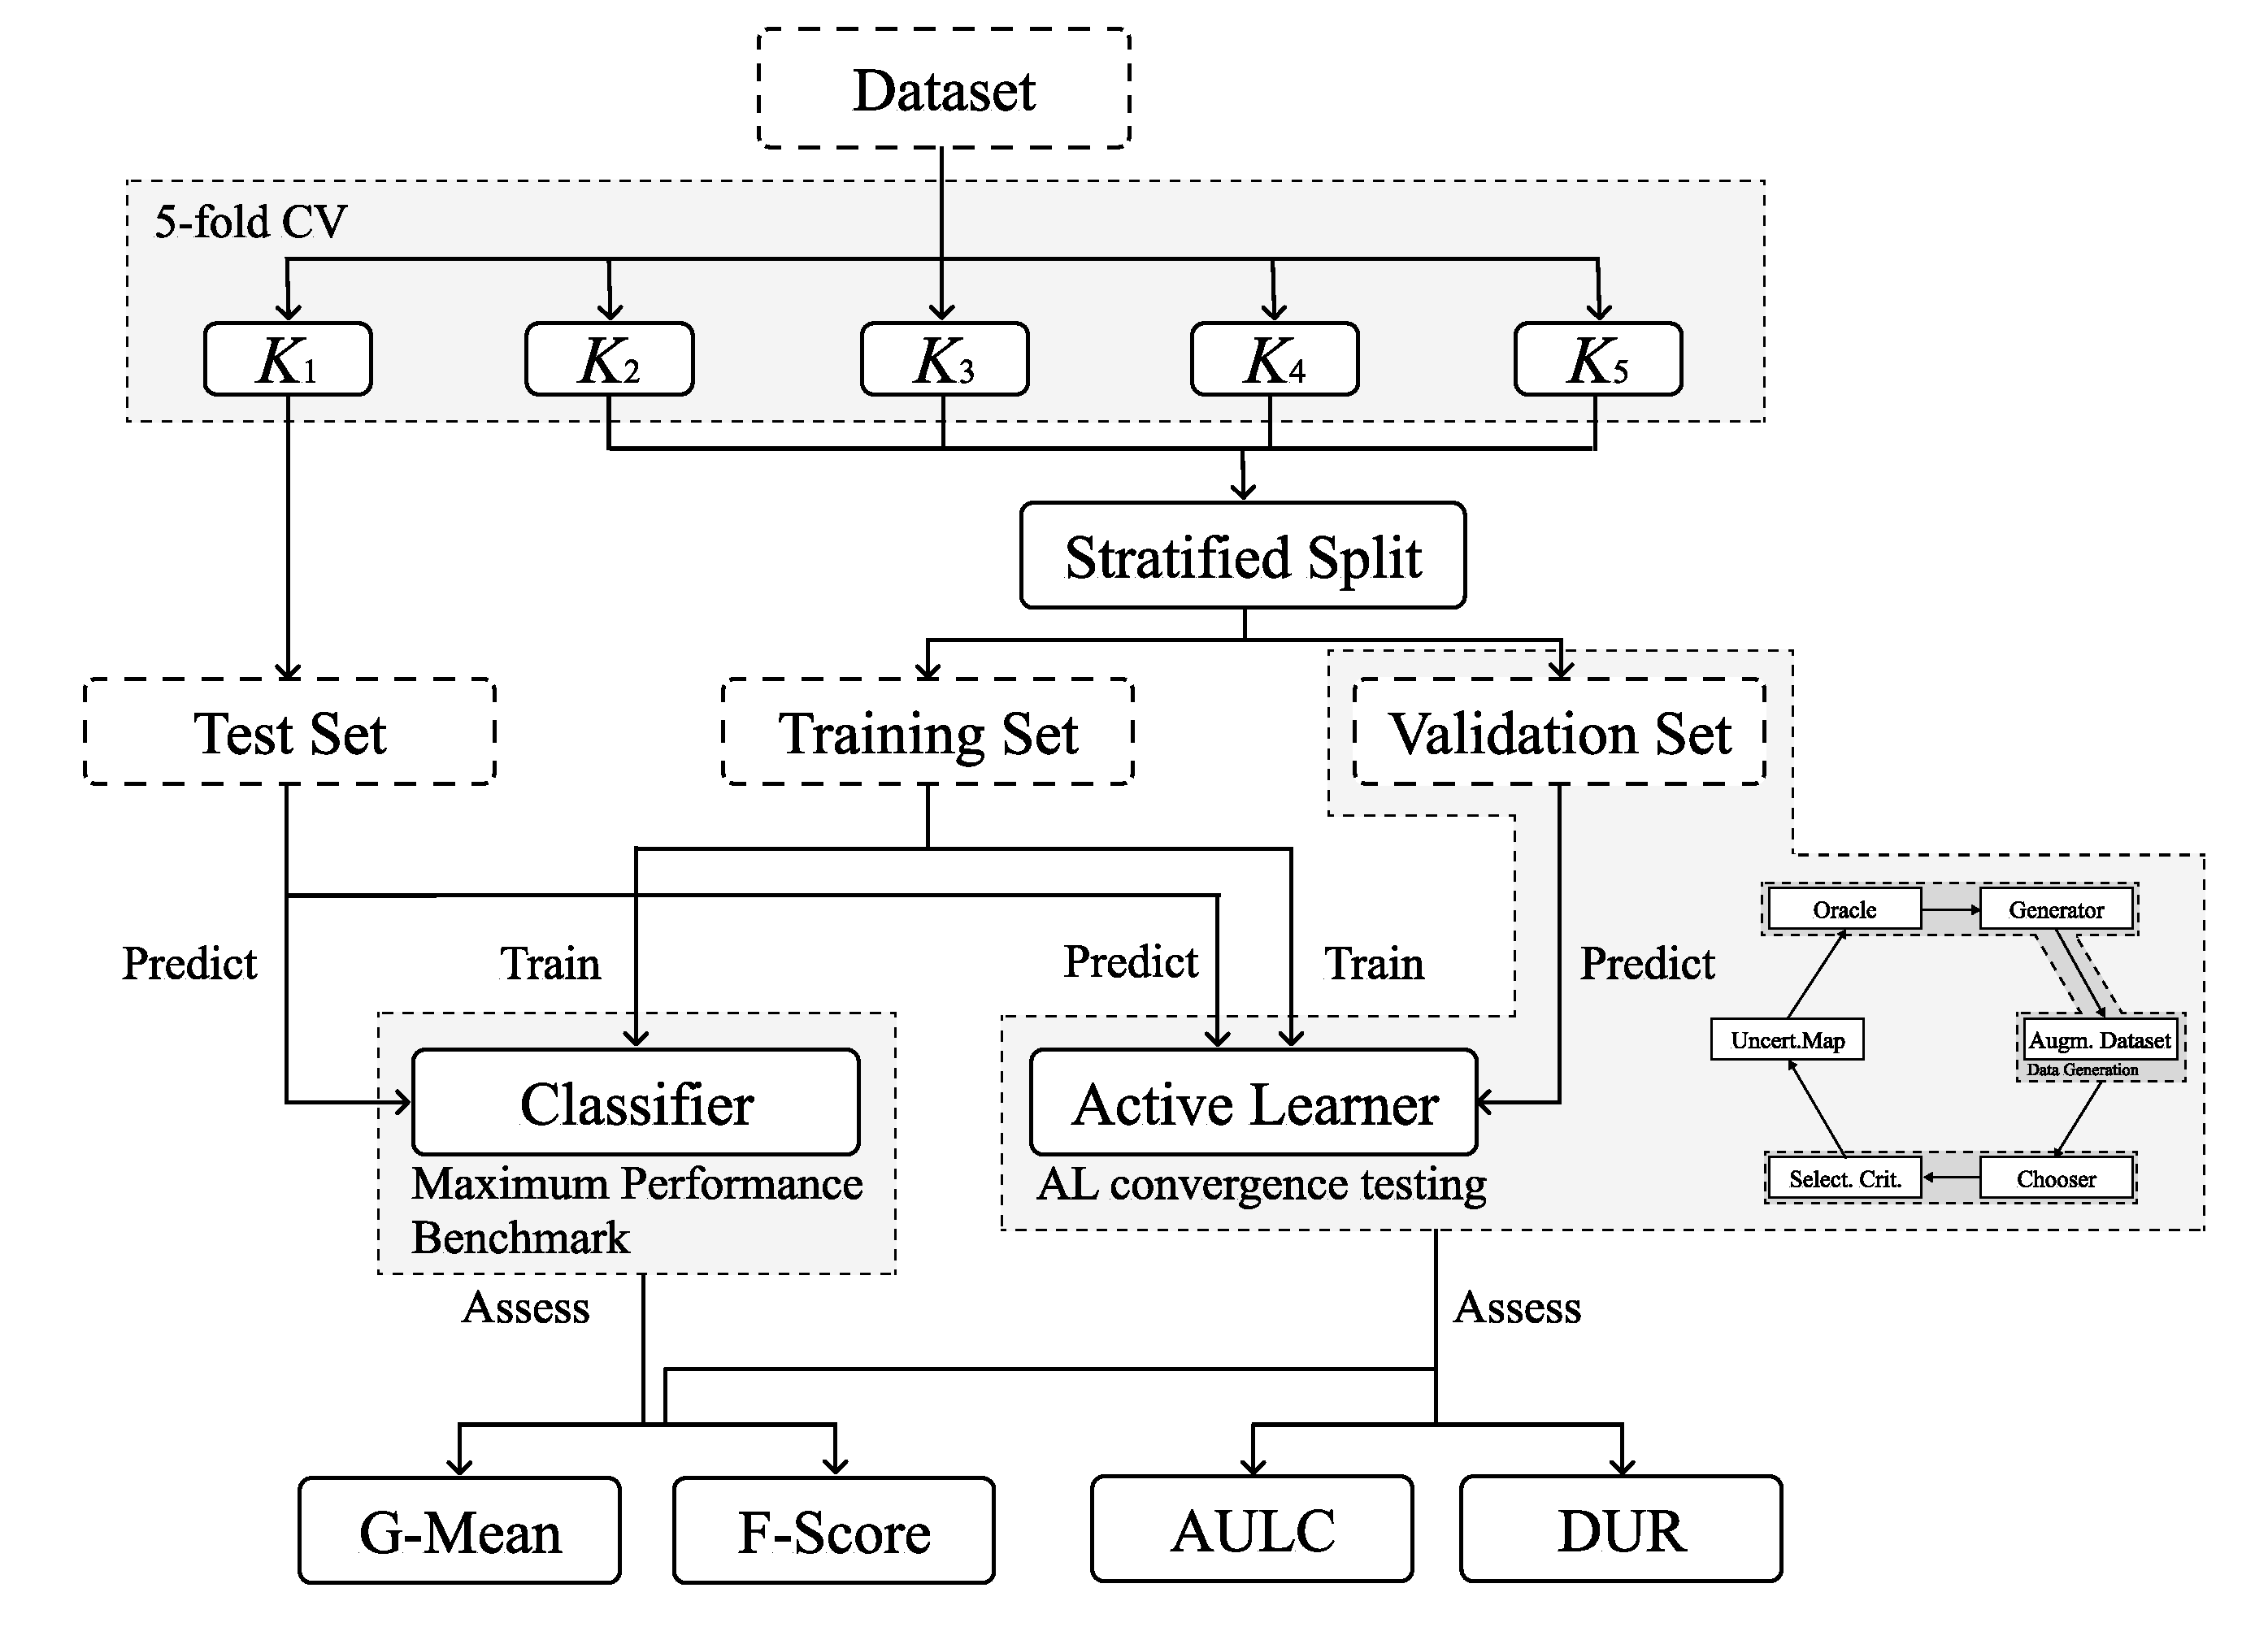
\includegraphics[width=.75\linewidth]{../analysis/experiment_pipeline}
    \caption{
        Experimental procedure. The datasets extracted from hyperspectral
        scenes are split in 5 folds. 1 of those (\textit{e.g.}, $K_1$) is used
        to test the optimal performance of AL algorithms and the
        classification without AL. The training set is used to iterate AL
        algorithms and train classifiers. The validation set is used to test
        the convergence of AL algorithms. The results are averaged over the 5
        folds across each of the 3 different initializations of this
        procedure.
    }~\label{fig:experiment_pipeline}
\end{figure}
\begin{paracol}{2}
\linenumbers
\switchcolumn

To make the AL-specific metrics comparable among active learners, the
configurations of the different frameworks must be similar. For each dataset,
the number of instances is constant to facilitate the analysis of the same
metrics. 

In most practical AL applications it is assumed that the number of instances 
in the initial training sample is too small to perform hyperparameter tuning.
Consequently, in order to ensure realistic results, our experimental procedure
does not include hyperparameter optimization. The predefined hyperparameters
are shown in Table~\ref{tab:grid}. They were set up based on general
recommendations and default settings for the classifiers and generators used.

The AL iterative process is set up with a randomly selected initial training
sample with 15 initial samples. At each iteration, 15 additional samples are
added to the training set. This process is stopped after 49 iterations, once
50\% of the entire dataset (\textit{i.e.,} 78\% of the training set) is added
to the augmented dataset.

\begin{table}[H]
	\centering
	\begin{tabular}{lll}
		\toprule
		Classifier & Hyperparameters      & Values             \\
		\midrule
		LR         & maximum iterations   & 10000              \\
		           & solver               & sag                \\
                   & penalty              & None               \\
		KNN        & \# neighbors         & 5                  \\
                   & weights              & uniform            \\
                   & metric               & euclidean          \\
		RF         & maximum tree depth   & None               \\
		           & \# estimators        & 100                \\
                   & criterion            & gini               \\
		\toprule
		Generator  &                      &                    \\
		\midrule
		G-SMOTE    & \# neighbors         & 5                  \\
                   & deformation factor   & 0.5                \\
                   & truncation factor    & 0.5                \\
		\bottomrule
	\end{tabular}
    \caption{\label{tab:grid}Hyper-parameter definition for the classifiers and
    generator used in the experiment.}
\end{table}

\subsection{Software Implementation}

The experiment was implemented using the Python programming language, along
with the Python libraries
\href{https://scikit-learn.org/stable/}{Scikit-Learn}~\cite{Pedregosa2011},
\href{https://imbalanced-learn.org/en/stable/}{Imbalanced-Learn}~\cite{JMLR:v18:16-365},
\href{https://geometric-smote.readthedocs.io/en/latest/?badge=latest}{Geometric-SMOTE},
\href{https://cluster-over-sampling.readthedocs.io/en/latest/?badge=latest}{Cluster-Over-Sampling}
and
\href{https://research-learn.readthedocs.io/en/latest/?badge=latest}{Research-Learn}
libraries. All functions, algorithms, experiments and results are provided in
the \href{https://github.com/joaopfonseca/research/}{GitHub repository of the
project}.

\section{Results \& Discussion}~\label{sec:results}

The evaluation of the different AL frameworks in a multiple dataset context
should not rely uniquely on the mean of the performance metrics across
datasets.~\cite{demvsar2006} recommends the use of mean ranking scores, since
the performance levels of the different frameworks varies according to the
data it is being used on. Consequently, evaluating these performance metrics
solely based on their mean values might lead to inaccurate analyses.
Accordingly, the results of this experiment are analysed using both the mean
ranking and absolute scores for each model. The rank values are assigned based
on the mean scores resulting from three different initializations of 5-fold
cross validation for each classifier and active learner. The goal of this
analysis is to understand whether the proposed framework (AL with the
integration of an artificial data generator) is capable of using less data
from the original dataset while simultaneously achieving better classification
results than the standard AL framework, \textit{i.e.}, guarantee a faster
classification convergence. 

\subsection{Results}~\label{sec:sub_results}

Table~\ref{tab:aulc_ranks} shows the average rankings and standard deviations
across datasets of the AULC scores for each active learner.

\begin{table}[H]
    \centering
    \pgfplotstabletypeset[
        col sep=comma,
        string type,
        every head row/.style={%
            before row=\toprule,
            after row=\midrule
        },
        every last row/.style={after row=\bottomrule},
    ]{../analysis/mean_std_aulc_ranks.csv}
    \caption{
        Mean rankings of the AULC metric over the different datasets (7),
        folds (5) and runs (3) used in the experiment. This means that the use
        of G-SMOTE always improves the results of the original framework.
    }\label{tab:aulc_ranks}
\end{table}

The mean AULC absolute scores are provided in Table~\ref{tab:aulc_scores}.
These values are computed as the mean of the sum of the scores of a specific
performance metric over all iterations (for an AL configuration). In other
words, these values correspond to the average AULC over $7\ datasets \times 5\
folds \times 3\ initializations$.

\begin{table}[htb]
    \centering
    \pgfplotstabletypeset[
        col sep=comma,
        string type,
        every head row/.style={%
            before row=\toprule,
            after row=\midrule
        },
        every last row/.style={after row=\bottomrule},
    ]{../analysis/mean_std_aulc_scores.csv}
    \caption{\label{tab:aulc_scores}
        Average AULC of each AL configuration tested. Each AULC score is
        calculated using the G-mean scores of each iteration in the validation
        set. By the end of the iterative process, each AL configuration used a
        total of 750 instances of the 960 instances that compose the training
        set.
    }
\end{table}

The average DURs are shown in Table~\ref{tab:optimal_data_utilization}. They
were calculated for various G-mean scores thresholds, varying at a step of 5\%
between 60\% and 95\%. Each row shows the percentage of training data required
by the different AL configurations to reach that specific G-mean score.

\end{paracol}
\captionsetup{justification=centering}
\pgfplotstabletypeset[
	begin table=\begin{longtable},
	end table=\end{longtable},
	col sep=comma,
	header=true,
    columns={Performance,Classifier,Standard,Proposed}, 
    string type,
    every head row/.style={before row=\toprule, after row=\midrule\endhead},
	every last row/.style={
        after row={
            \bottomrule
            \caption{
                Mean data utilization of AL algorithms, as a percentage of the training set.
            }\label{tab:optimal_data_utilization}
        }
    }
]{../analysis/optimal_data_utilization.csv}
\begin{paracol}{2}
\linenumbers
\switchcolumn



The averaged optimal classification scores are shown in
Table~\ref{tab:optimal_mean_std_scores}. The maximum performance (MP)
classification scores are shown as a benchmark and represent the performance
of the corresponding classifier using the entire training set. 

\begin{table}[htb]
    \centering
    \addtolength{\leftskip} {-2cm}
    \addtolength{\rightskip}{-2cm}
    \pgfplotstabletypeset[
        col sep=comma,
        string type,
        every head row/.style={%
            before row=\toprule,
            after row=\midrule
        },
        every last row/.style={after row=\bottomrule},
    ]{../analysis/optimal_mean_std_scores.csv}
    \caption{\label{tab:optimal_mean_std_scores}
        Optimal classification scores. The Maximum Performance (MP)
        classification scores are calculated using classifiers trained using
        the entire training set.
    }
\end{table}

\subsection{Statistical Analysis}~\label{sec:statistical-analysis}

The methods used to test the experiment's results must be appropriate for a
multi-dataset context. Therefore the statistical analysis is performed using
the Wilcoxon signed-rank
test~\cite{Wilcoxon1945} as a post-hoc analysis. The variable used for this
test is the data utilization rate, considering the various performance
thresholds from Table~\ref{tab:optimal_data_utilization}.

The Wilcoxon signed-rank test results are shown in
Table~\ref{tab:wilcoxon_test}. We test as null hypothesis that the performance
of the proposed framework is the same as the original AL framework. The null
hypothesis was rejected in all datasets.

\begin{table}[htb]
	\centering
    \pgfplotstabletypeset[
        col sep=comma,
        string type,
        every head row/.style={%
            before row=\toprule,
            after row=\midrule
        },
        every last row/.style={after row=\bottomrule},
    ]{../analysis/wilcoxon_test.csv}
    \caption{
    	Adjusted p-values using the Wilcoxon signed-rank method. Bold values
        are statistically significant at a level of $\alpha = 0.05$. The 
        null hypothesis is that the performance of the proposed
        framework is similar to that of the original framework.
    }\label{tab:wilcoxon_test}
\end{table}

\subsection{Discussion}

This paper expands the AL framework by adding an artificial data generator
into its iterative process. This modification is done to accelerate the
classification convergence of the standard AL procedure, which is
reflected in the reduction of the amount of data necessary to reach better
classification results.

The convergence efficiency of the proposed method is always higher than the
baseline AL framework (NONE), as shown in Table~\ref{tab:aulc_ranks}. The AL
using data generation was able to outperform the baseline AL in all scenarios. 

The mean AULC scores in Table~\ref{tab:aulc_scores} show a significant
improvement in the performance of AL when a generator is used. The mean
performance of the proposed framework is always better than the
baseline framework. This improvement is explained by:

\begin{enumerate}
    \item Earlier convergence of AL, \textit{i.e.}, requiring less data to
        achieve comparable performance levels. This effect is shown in
        Table~\ref{tab:optimal_data_utilization}, where we found that the
        proposed framework always uses less data for similar performance
        levels, regardless of the classifier used.
    \item Higher optimal classification performance, \textit{i.e.}, reaching
        higher performance levels overall. This effect is studied in
        Table~\ref{tab:optimal_mean_std_scores}, where we found that using a
        generator in AL led to a better classification performance and was
        capable of outperforming the MP threshold. 
\end{enumerate} 

Our results show statistical significance in every dataset. The proposed
framework had a superior performance with statistical significance on each
dataset at a level of $\alpha = 0.05$. This indicates that regardless of the
context under which an AL algorithm is used, the proposed framework reduces
the amount of data necessary in the AL's iterative process.

This paper introduces the concept of applying data a generation algorithm in
the AL framework. This was done with the implementation of a recent state of
the art generalization of a popular data generation algorithm. Although, since
this algorithm is based on heuristics, future work should focus on improving
these results through the design of new data generation mechanisms, at the
cost of additional computational power. In addition, we also noticed
significant standard errors in our experimental results
(see Subsection~\ref{sec:sub_results}). This indicates that
AL procedures seem to be particularly sensitive to the initialization method,
which is still a limitation of AL, regardless of the framework and
configurations used. This is consistent with the findings
in~\cite{Kottke2017}, which future work should attempt to address. Although
using a generator marginally reduced this standard error, it is not sufficient
to address this specific limitation.

\section{Conclusion}~\label{sec:conclusion}

The aim of this experiment was to test the effectiveness of a new AL framework
that introduces artificial data generation in its iterative process. The
experiment was designed to test the proposed method under particularly
challenging conditions, where the maximum performance line is naturally high
in most datasets. The element that constitute the Generator component was set
up in a plug-and-play scheme, without significant tuning of the G-SMOTE
oversampler. Using a generator in AL improved the original AL framework in all
scenarios. These results could be further improved through the modification
and more intense tuning of the data generation strategy. In our experiment,
artificial data was generated only to match each non-majority class frequency
with the majority class frequency, strictly balancing the class distribution.
Generating a larger amount of data for all classes can further improve these
results. 

The high performance scores for the baseline AL framework made the achievement
of significant improvements over the traditional AL framework under these
conditions particularly meaningful. The advantage of the proposed AL framework
is shown in Table~\ref{tab:optimal_data_utilization}. In most of the presented
scenarios there is a substantial reduction of data necessary to reach a given
performance threshold. 

The results from this experiment show that using a data generator in the AL
framework will improve the convergence of the method. This framework
successfully anticipate the predictor's optimal performance, as shown in
Tables~\ref{tab:aulc_ranks},~\ref{tab:aulc_scores}
and~\ref{tab:optimal_data_utilization}. Therefore, in a real application, the
annotation cost would have been reduced since less iterations and labeled
instances are necessary to reach near optimal classification performance.

\acknowledgments{
    The authors would like to thank Professor Victor Lobo (NOVA IMS,
    Universidade Nova de Lisboa, and CINAV, Escola Naval, CIDIUM) for
    reviewing this paper and providing important feedback throughout its
    development.
}

\authorcontributions{
    Conceptualization, F.B.; Methodology, J.F. and G.D.; Software, J.F. and
    G.D.; Validation, F.B., G.D.; Formal Analysis, J.F; Writing - Original
    Draft Preparation, J.F.; Writing - Review \& Editing, F.B., G.D., J.F.;
    Supervision, F.B.; Funding Acquisition, F.B.
}

\funding{
    This research was funded by ``Fundação para a Ciência e a Tecnologia''
    (Portugal) [grant numbers PCIF/SSI/0102/2017 - foRESTER,
    DSAIPA/AI/0100/2018 - IPSTERS].
}

\dataavailability{
    The data reported in this study is publicly available. It can be retrieved
    and preprocessed using the Python source code provided at
    \url{https://github.com/joaopfonseca/research}. Alternatively the original
    data is available at
    \url{http://www.ehu.eus/ccwintco/index.php?title=Hyperspectral_Remote_Sensing_Scenes}.
} 

\conflictsofinterest{
    The authors declare no conflict of interest. The funders had no role in
    the design of the study; in the collection, analyses, or interpretation of
    data; in the writing of the manuscript, or in the decision to publish the
    results.
}

\end{paracol}

\reftitle{References}
\externalbibliography{yes}
\bibliography{references}

\end{document}
